\documentclass{article}
\usepackage[a4paper, total={7in, 10in}]{geometry}
\usepackage{fontspec} 
\usepackage{xeCJK} 
\setCJKmainfont{標楷體}
\setmainfont{Times New Roman}
\XeTeXlinebreaklocale “zh” 
\XeTeXlinebreakskip = 0pt plus 1pt
\usepackage{graphicx}
\usepackage{float}
\usepackage{xcolor}
\usepackage[linesnumbered,ruled,vlined]{algorithm2e}
\usepackage{mathtools}
\usepackage{amsmath} 
\usepackage{subfigure}  




\newcommand\mycommfont[1]{\footnotesize\ttfamily\textcolor{blue}{#1}}
\SetCommentSty{mycommfont}

\SetKwInput{KwInput}{Input}                % Set the Input
\SetKwInput{KwOutput}{Output}              % set the Output

\title{Self-Driving Cars(Mid)}
\author{309611087 洪得瑜}
\date{2022 11/17} 

\begin{document}
\maketitle
\section{ITRI.bag}
ITRI bag 實際流程如圖\ref{fig:itri.png}所示,在ITRI bag 中啟動ROS後建立共三個節點高精地圖、GPS及光達頂雲圖,在近入光達節點後需確定第一次GPS及高精地圖是否Ready,若為false則等待0.05秒後進入雲點圖姿態及位置估算,當進入點雲估算時先對點雲圖進行降採樣有助於降低雲點數量及提高匹配皆設定為1.0,完成降採樣後進行雲點初值估測,而第一步的位置採用GPS作為trasn設定,而初始姿態無法從感測得知因此在此採旋轉360度,尋找當中由ICP估測後的最小值,在此我以10度為單位收斂設為10次加快尋找,找到大概姿態後進行第一次的NDT定位,而在ITRI bag中我使用兩種點雲演算法ICP及NDT進行比較,最終將點雲圖估測後姿態位置儲存下一次初始設定,並將結果發布及儲存,在進行下一步估測值到bag資料結束。
\begin{figure}[H]
\centering
	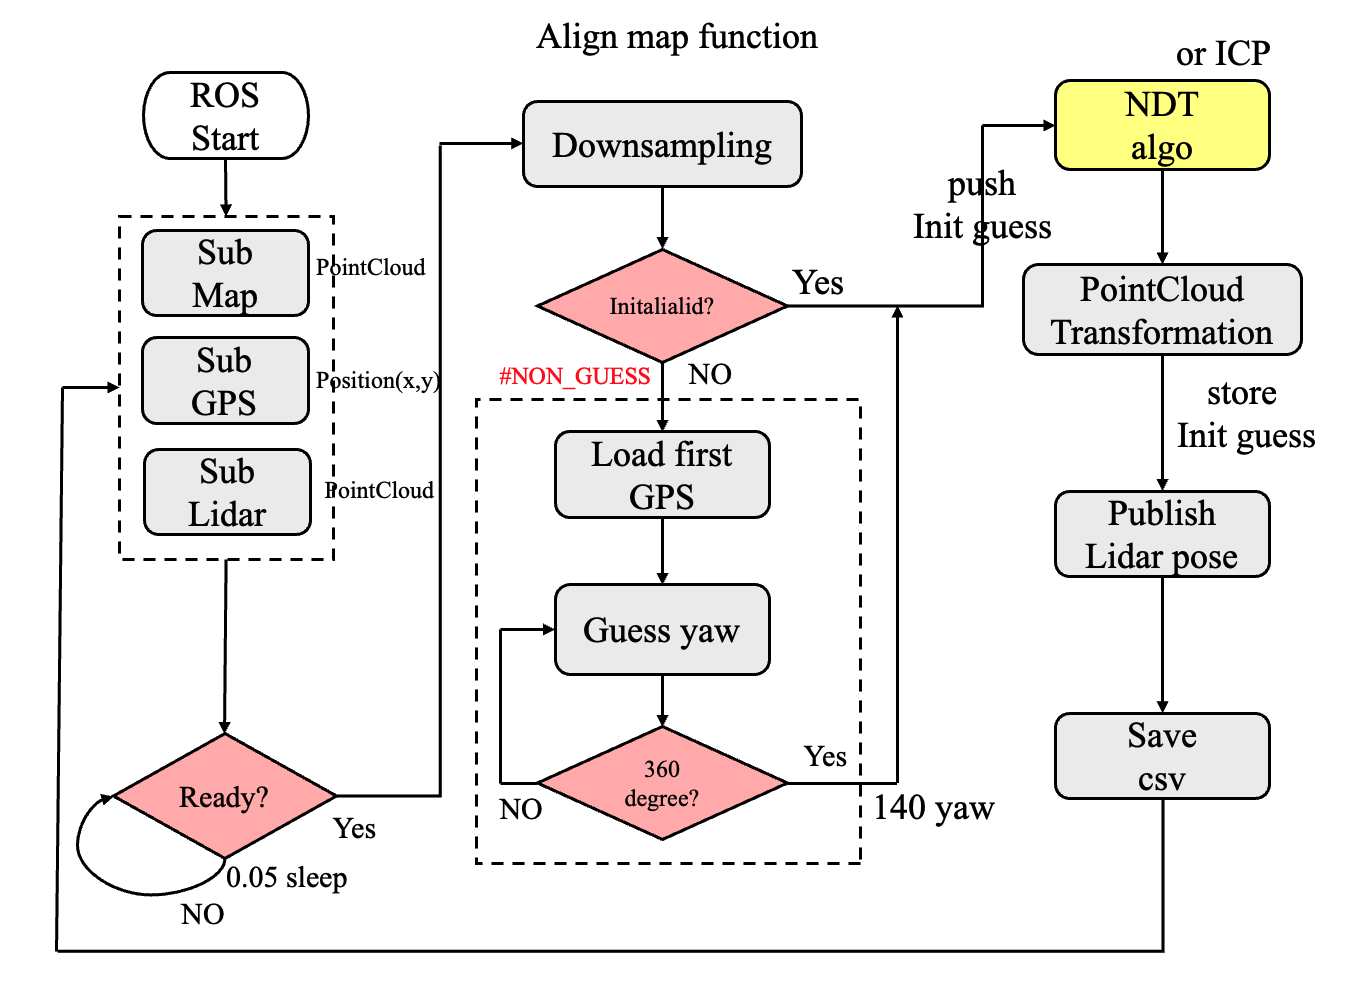
\includegraphics[width=0.8\textwidth]{./ITRI_flow.png}
	\caption{ITRI流程圖}
	\label{fig:itri.png}
\end{figure}


\section{nuScenes2/3.bag}
nuScenes2/3可由ITRI基礎流程做改變,在此增加新節點Wheel odom 及 IMU 感測資料進行融合使用Strapdown估測姿態矩陣及位置估測較佳的初始值提高精準度。
\begin{figure}[H]
\centering
	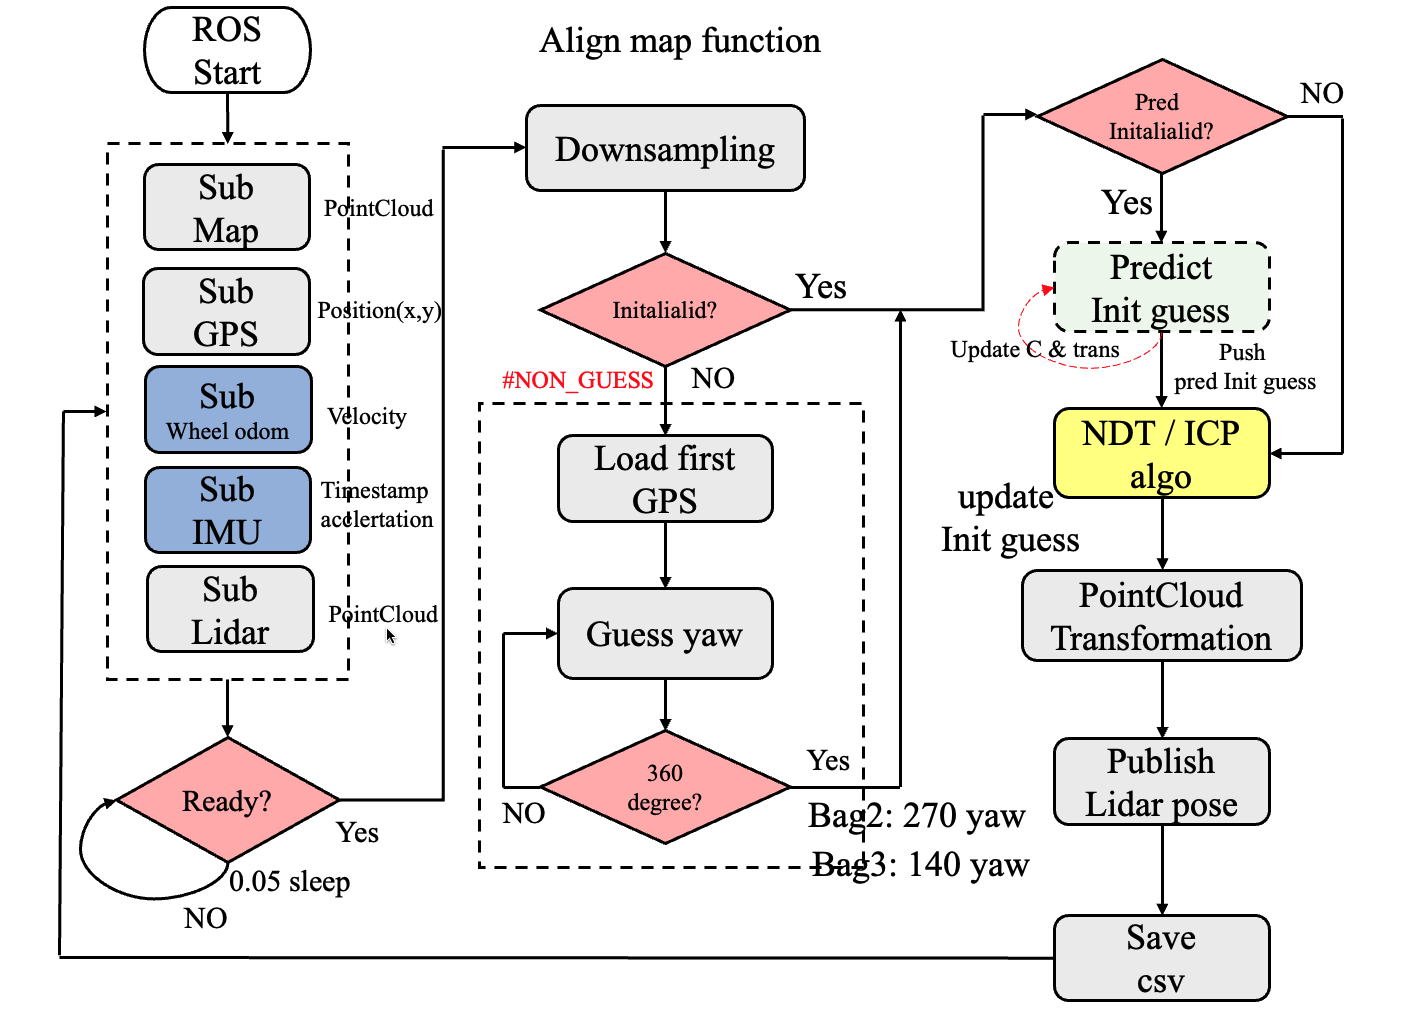
\includegraphics[width=0.8\textwidth]{./nuscenes.png}
	\caption{nuScenes流程圖}
	\label{fig:.png}
\end{figure}
\subsection{Pred Init guess}
估測方法參考文獻\cite{1}中以角速度方法估測更新下一次姿態矩陣,及經由IMU加速度預測下一時刻位置,並融合wheel odom定時更新速度,降低因由IMU積分所造成的誤差,由估測方法可使Init guess更接近ground truth在ICP上有相當大的精準度提升,實際對應程式如下介紹。
\subsubsection{Tracking Orientation Implementaion}
由\cite{1}中提及C(t)定義為為姿態旋轉矩陣,而IMU提供非連續信號$\omega$因此以積分採樣信號,短時距下變化$\delta{t}$可提供足夠應用而\cite{1}使用rectangular rule計算出B矩陣,而根據當前角速度推測$\delta{t}$變化下,推測下一極小時刻姿態,而當中的$\sigma=|\omega_b \delta{t}|$為角速度norm乘上短時間絕對值,預測姿態結果為$C(t+\delta{t})$計算過程如下所示。

\begin{equation}
	C(t+\delta{t}) - C(t)\cdot exp(\int_{t}^{t+\delta t} \Omega(t)dt)
\end{equation}

\begin{equation}
	\int_{t}^{t+\delta{t}}\Omega(t)dt=B
\end{equation}

\begin{equation}
	B = \begin{pmatrix} 0 & -\omega_{bz}\delta{t} & \omega_{by}\delta{t}\\
						\omega_{bz}\delta{t} & 0 & -\omega_{bx}\delta{t}\\
						-\omega_{by}\delta{t} & \omega_{bx}\delta{t} & 0
		\end{pmatrix}
\end{equation}

\begin{equation}
	C(t+\delta{t})=C(t)\left(I+B+\frac{B^2}{2!} + \frac{B^3}{3!} + \frac{B^4}{4!} + ... \right)
\end{equation}

\begin{equation}
 	= C(t)\left(I + B + \frac{B^2}{2!} - \frac{\sigma^2B}{3!} - \frac{\sigma^2B^2}{4!} + ... \right)
\end{equation}

\begin{equation}
	= C(t)\left(I + \left( 1 - \frac{\sigma^2}{3!} + \frac{\sigma^4}{5!}... \right)B + \left(\frac{1}{2!} - \frac{\sigma^2}{4!} + \frac{\sigma^4}{6!}...\right)B^2 \right)
\end{equation}

\begin{equation}
	=C(t)\left(I + \frac{sin\sigma}{\sigma}B+\frac{1-cos\sigma}{\sigma^2}B^2 \right)
\end{equation}

\subsubsection{Tracking Position Implementaion}
文獻\cite{1}追蹤位置方法需先將IMU座標下加速度投影到以世界座標系統下(8),而可由姿態矩陣乘上加速度投影到世界座標下減去重力所造成的影響,由於積分的結果忽略重力所造成影響誤差將會累積過大,而在世界座標下後利用運動學公式推測下短時間位置$s_g(t+\delta{t})$。

\begin{equation}
	a_g(t) = C(t)a_b(t)
\end{equation}

\begin{equation}
	v_g(t) = v_g(0) + \int_0^ta_g(t)-g_g dt
\end{equation}

\begin{equation}
 	s_g(t) = s_g(0) + \int_0^tv_g(t)dt
\end{equation}

\begin{equation}
	\begin{cases}
		v_g(t+\delta{t}) = v_g(t) + \delta{t} \cdot (a_g(t+\delta{t})- g_g)\\
		s_g(t+\delta{t}) = s_g(t) + \delta{t} \cdot v_g(t+\delta{t})
	\end{cases}
\end{equation}

\subsubsection{Implement to Code}
由\cite{1}strapdown預測$\delta{t}$極小時間下姿態矩陣,而初始姿態矩陣C(t)由點雲圖匹配後計算的姿態給定,經由雲點圖計算後Init guess更新至C(0)旋轉矩陣,及更新新的位置狀態降低因IMU積分導致的誤差累積,而更新後的Init guess 透過IMU的感測資料$\omega$及加速度資訊更新$C(t+\delta{t})$,而車輛初速度透過wheel odom獲得,在為更新前由IMU加速度持續更新速度,當新的wheel odmo velocity更新至v0,而預測持續更新若需要做雲點圖時將當前估測作為Init guess,由於本次忽略z軸上估測因此$g=0$,感測器融合關係如圖\ref{fig:fuse.png}。
\begin{figure}[H]
\centering
	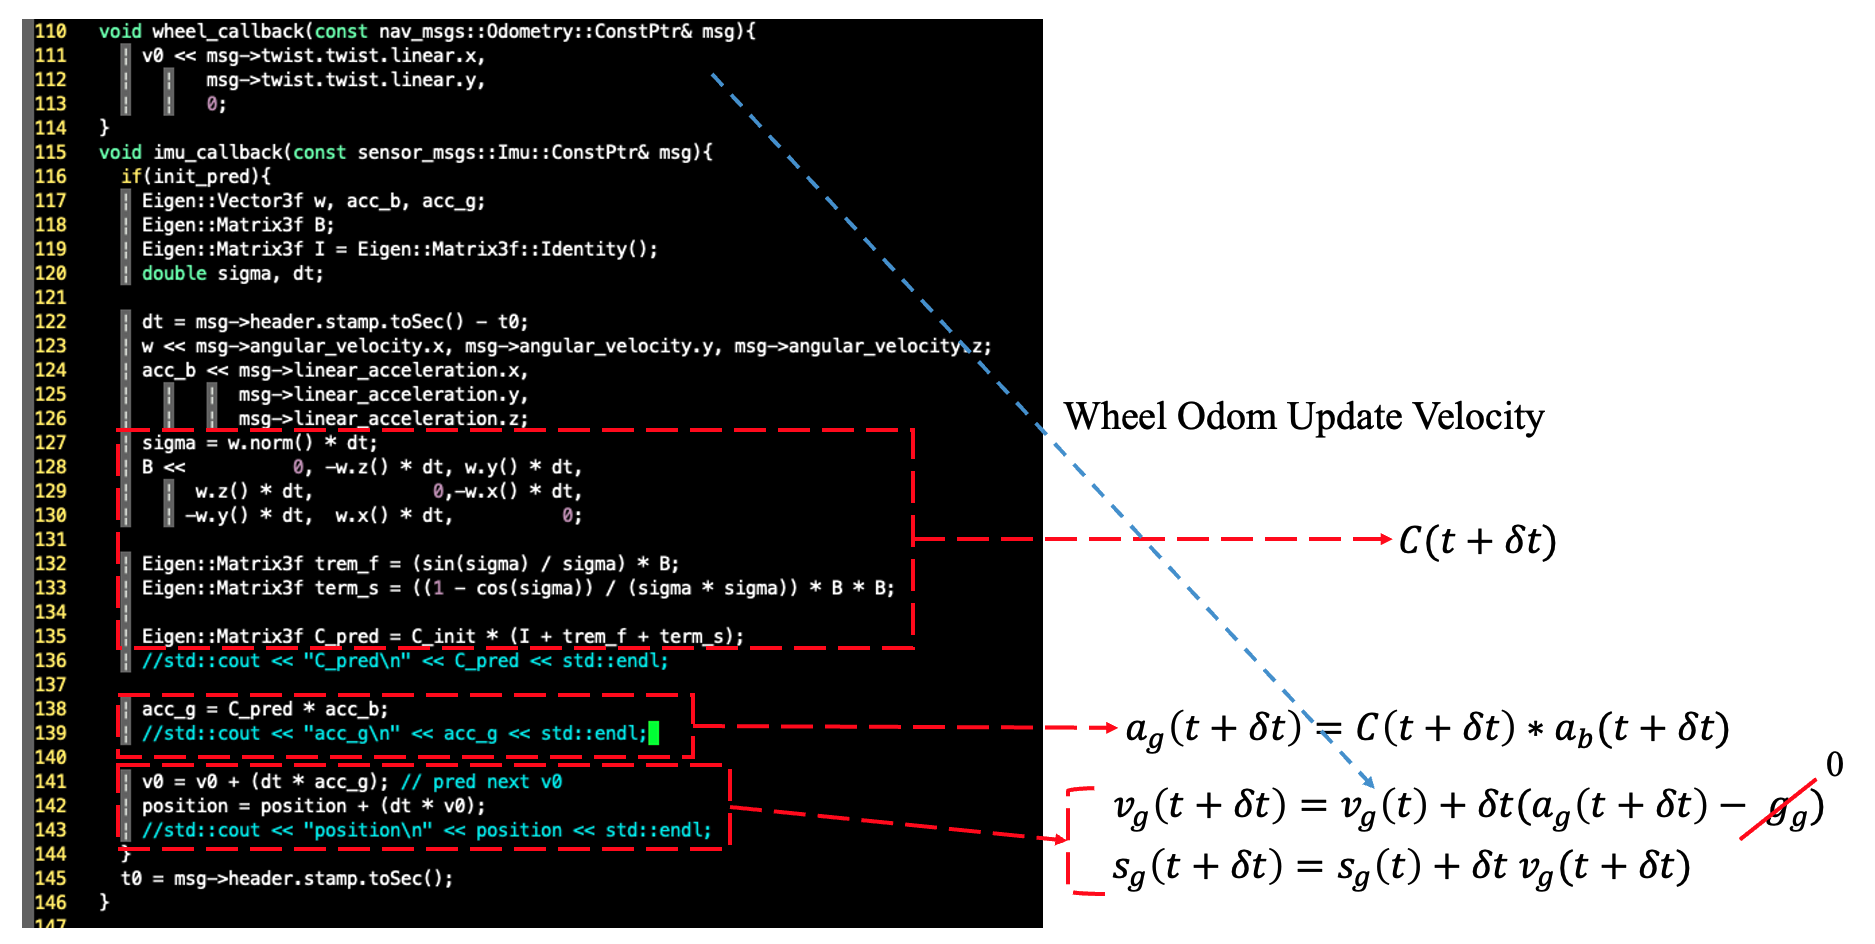
\includegraphics[width=1.0\textwidth]{./code.png}
\end{figure}

\begin{figure}[H]
\centering
	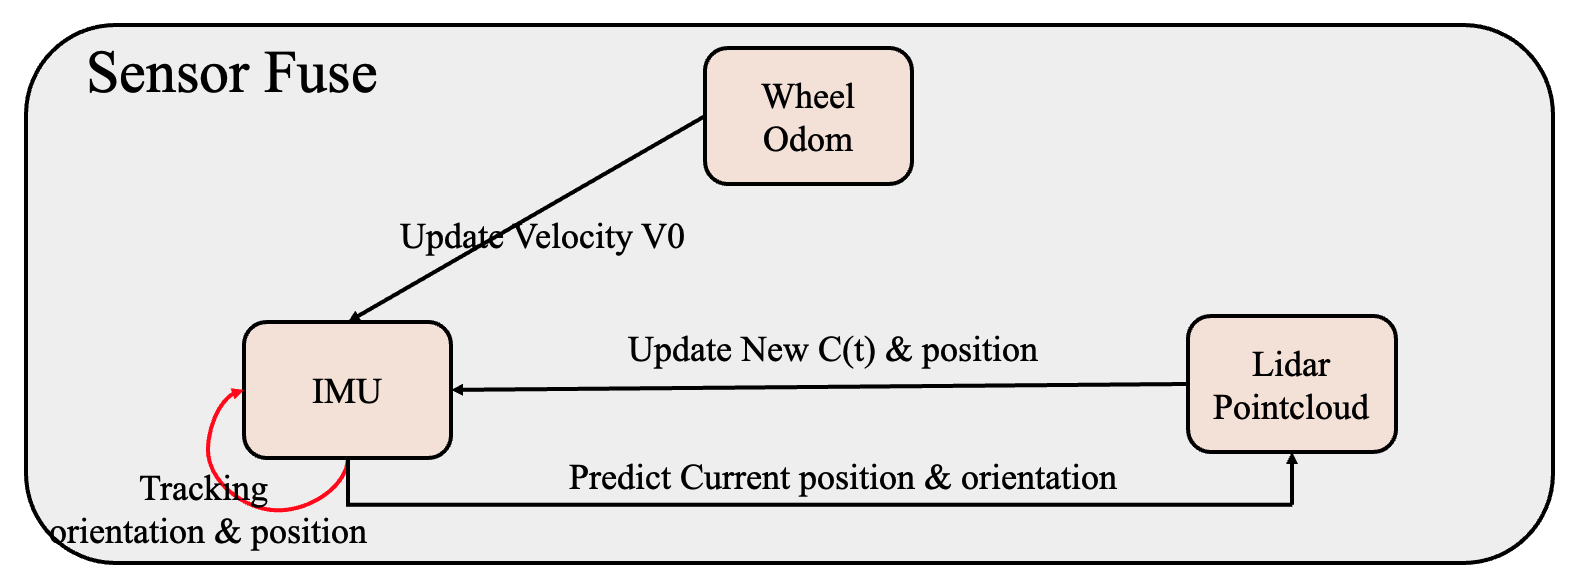
\includegraphics[width=0.8\textwidth]{./fuse.png}
	\caption{感測器融合關係圖}
	\label{fig:fuse.png}
\end{figure}

\section{Contribuition}
經由實際結果分析數據,本分析結果皆基於全程使用NDT結果視為ground truth 比較分析(由於無法取的的實際ground truth資料,而在kaggle NDT分數相較較低),因此我視為最接近ground truth 進行資料比對,根據不同bag分析結果如下。
\subsection{ITRI result}
ITRI以全程使用ICP及全程NDT進行比較分析,分析兩者差值共分析x,y,yaw三軸數據,在全使用ICP下kaggle sore 為0.0247而使用NDT方法可降至0.01396,結果顯示以不進行預測Init guess下使用ICP會有較大誤差,而在第一步以ICP下由於Init guess為概略位置導致起步位置誤差達20cm,而在120幀時進入轉彎ICP Init guess 若使用前一時刻進行估測位置誤差漸漸增加大約在5cm,而在yaw也增加到0.015,如圖\ref{fig:res1.png}所示。
\begin{figure}[H]
\centering
	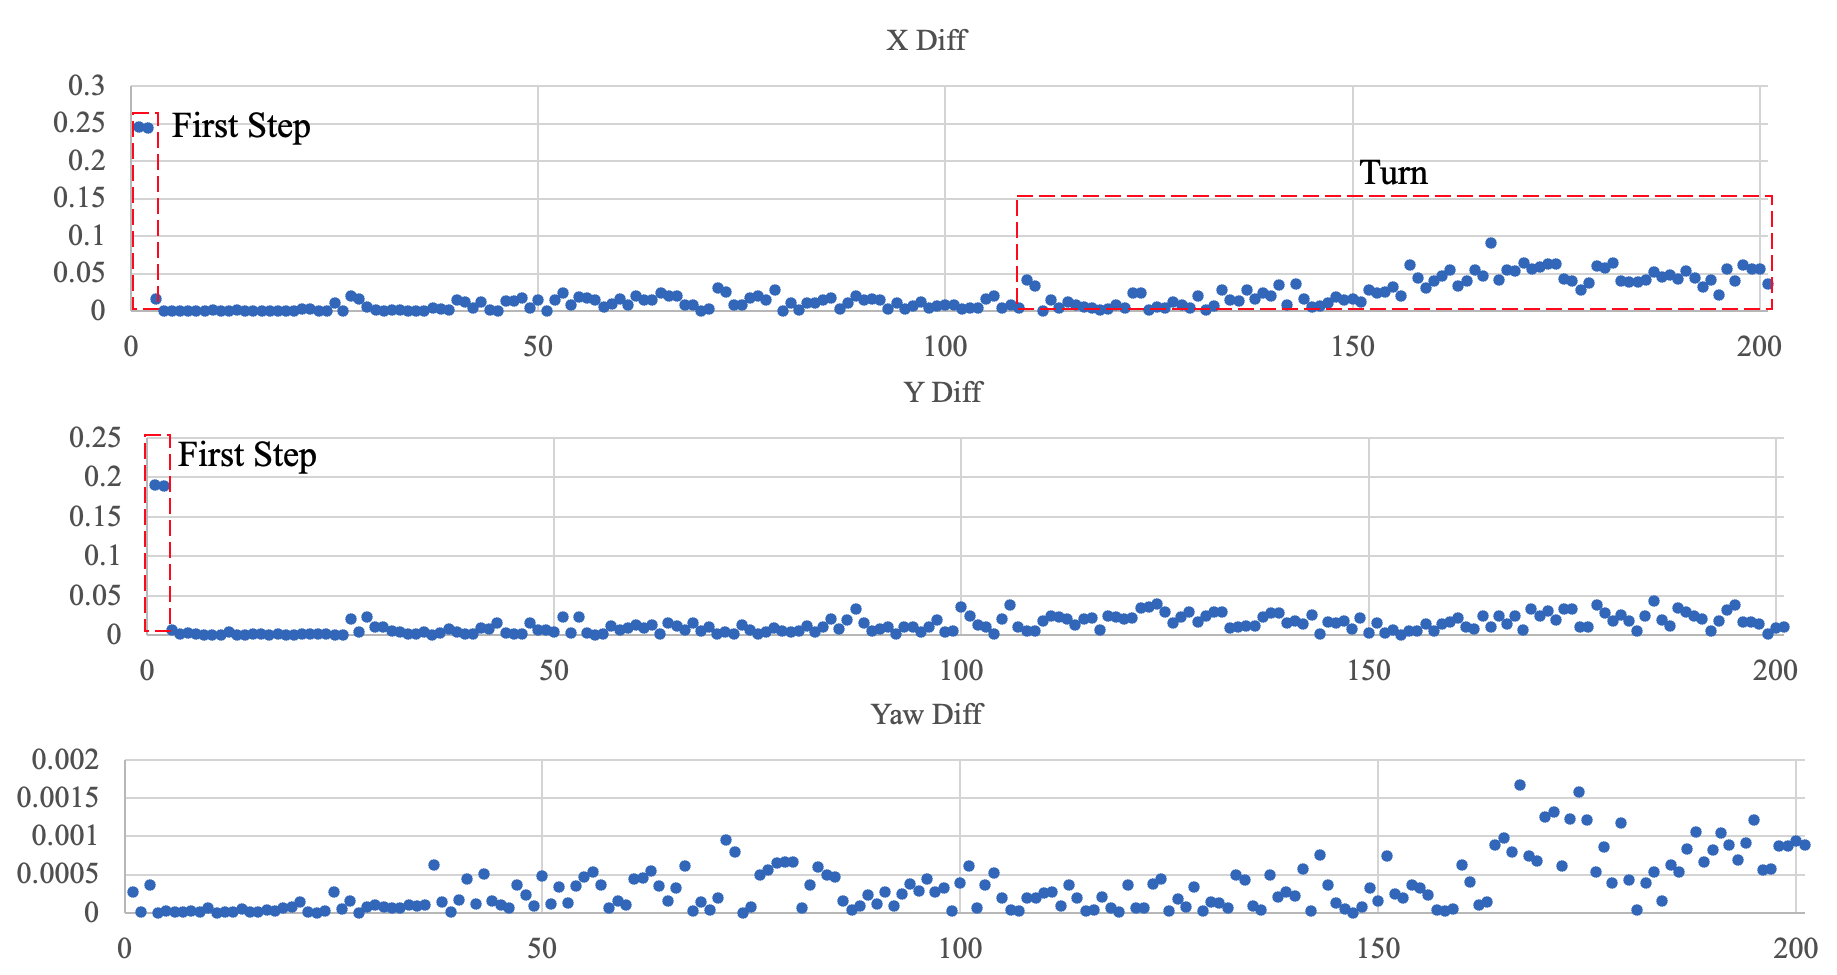
\includegraphics[width=0.8\textwidth]{./ITRI_res.png}
	\caption{ITRT Bag NDT減去ICP 各別x y yaw數據分析結果}
	\label{fig:res1.png}
\end{figure}
\subsection{nuScenes2 result}
由ITRI經驗可得到ICP方法需要較佳的Initt guess,若使用前一時刻作為Init guess計算出姿態及位置誤差較大,因此在此我增加IMU及wheel odmo 感測資料做tracking使init guess 更接近當前位置降低誤差,詳細方法如2.1.3所示,除此之外在ITRI中全程使用NDT方法計算時間過長,因此設計切換方法降低計算時間,第一步以NDT計算下一步使用ICP進行不斷切換,可降低一半時間且可有助於修正ICP結果提供更佳Init guess,分析結果如下所示。
\subsubsection{x 軸結果分析}
\begin{figure}[H]
\centering
	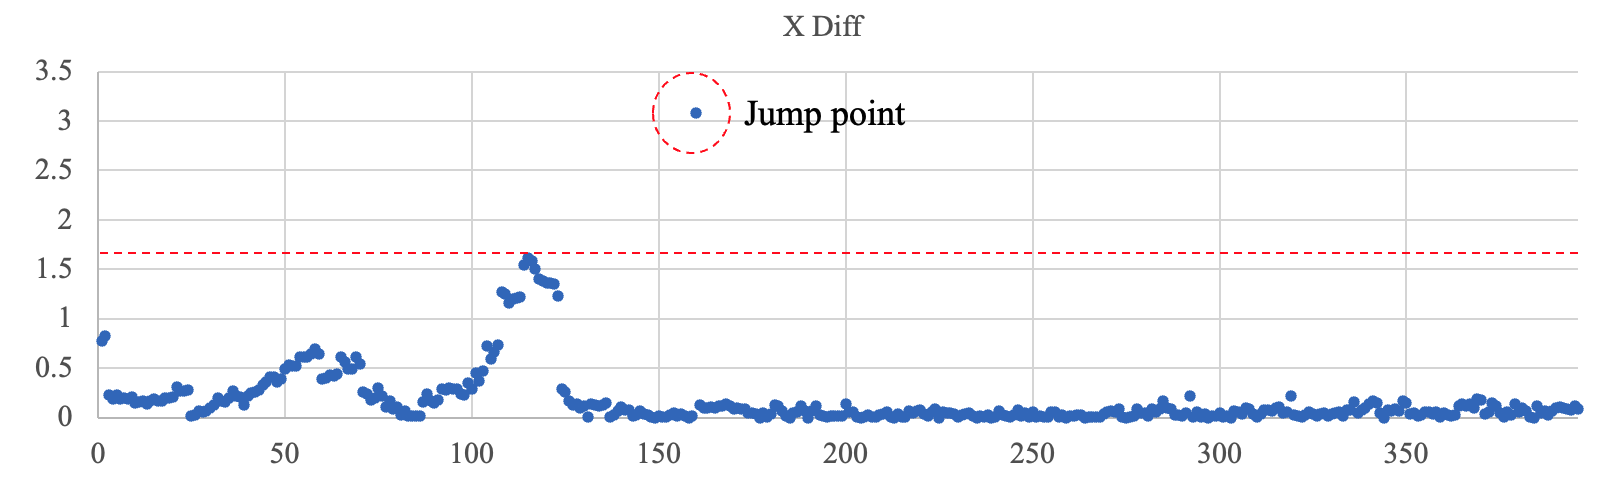
\includegraphics[width=0.8\textwidth]{./res2_x_icp.png}
	\caption{Bag2 NDT減去ICP 各別x軸數據分析結果}
\end{figure}

\begin{figure}[H]
\centering
	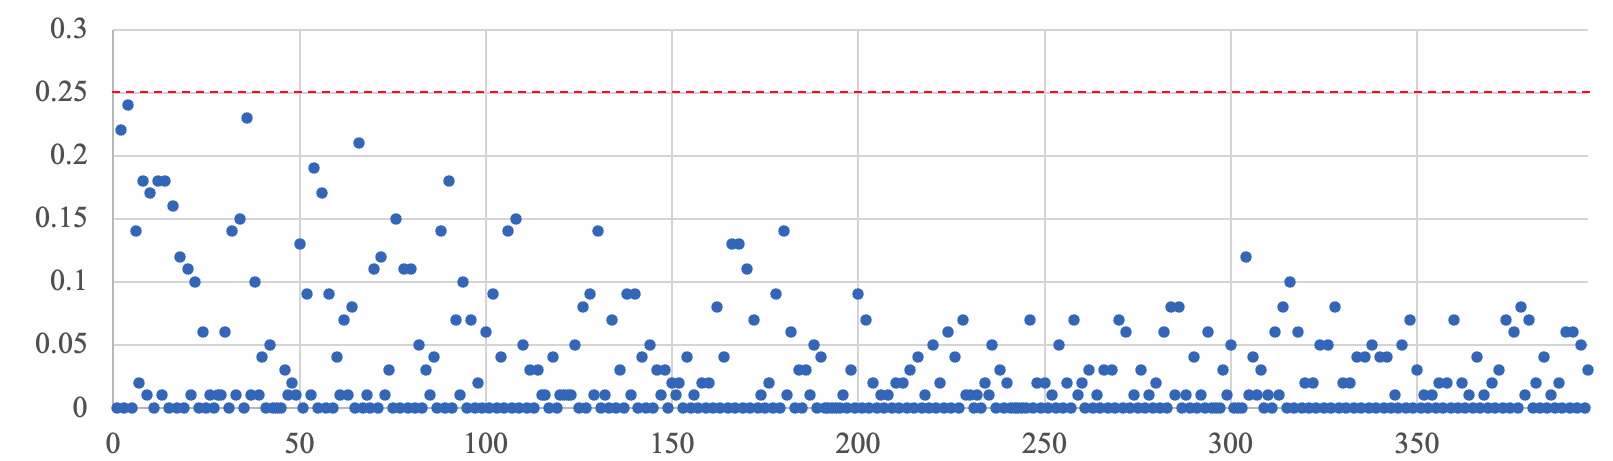
\includegraphics[width=0.8\textwidth]{./res2_x_icpndt.png}
	\caption{Bag2 NDT減去NDT及ICP切換方法 各別x軸數據分析結果(驗證有助於降低誤差)}
\end{figure}

\subsubsection{y 軸結果分析}

\begin{figure}[H]
\centering
	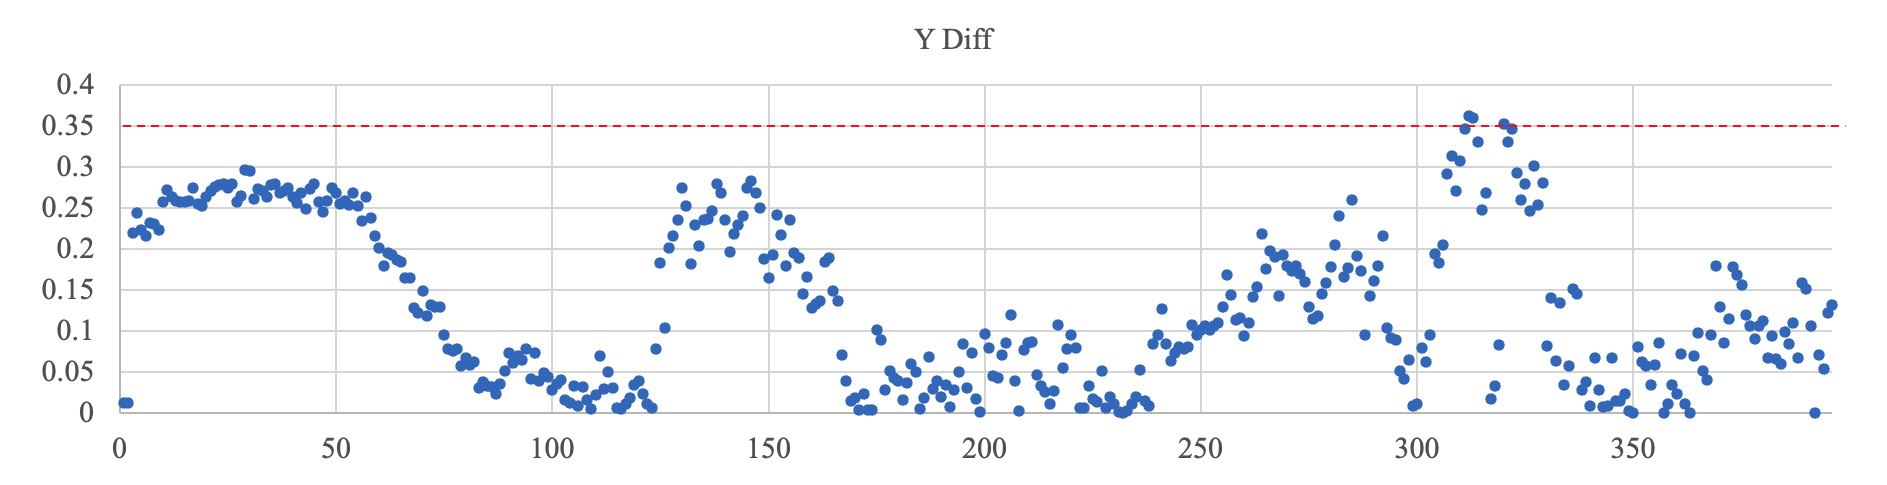
\includegraphics[width=0.8\textwidth]{./res2_y_icp.png}
	\caption{Bag2 NDT減去ICP 各別y軸數據分析結果}
\end{figure}

\begin{figure}[H]
\centering
	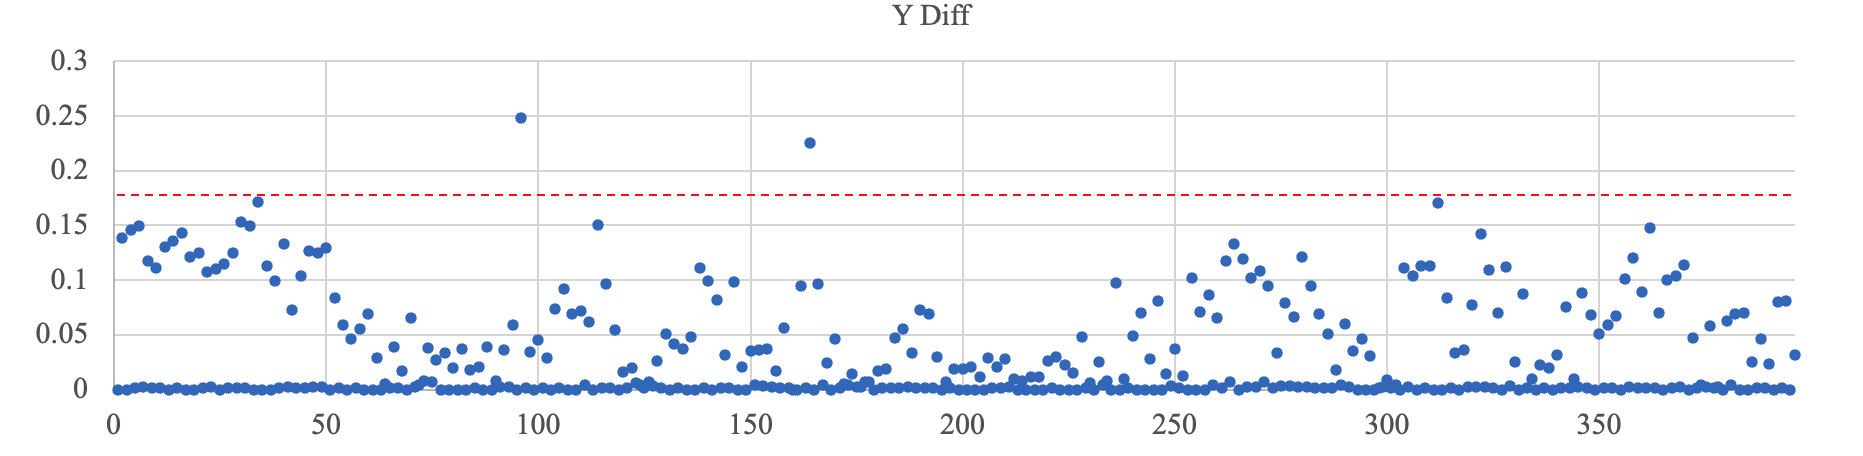
\includegraphics[width=0.8\textwidth]{./res2_y_icpndt.png}
	\caption{Bag2 NDT減去NDT及ICP切換方法 各別y軸數據分析結果(驗證有助於降低誤差)}
\end{figure}

\subsubsection{yaw 結果分析}
由於Bag2為直線前進因此yaw無明顯差異
\begin{figure}[H]
\centering
	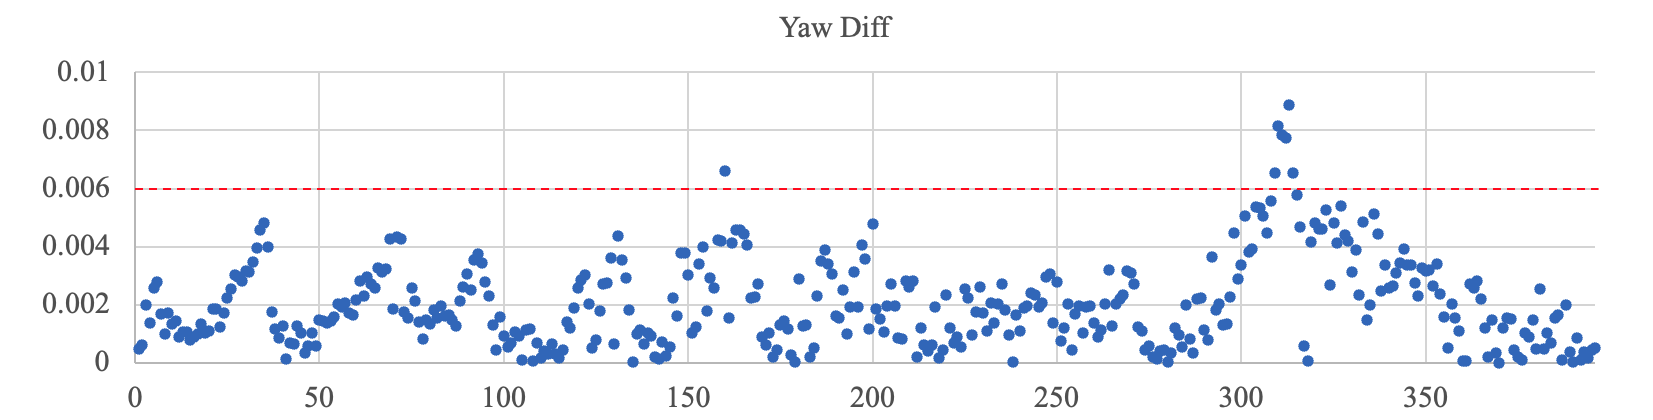
\includegraphics[width=0.8\textwidth]{./res2_icpyaw.png}
	\caption{Bag2 NDT減去ICP 各別yaw軸數據分析結果}
\end{figure}

\begin{figure}[H]
\centering
	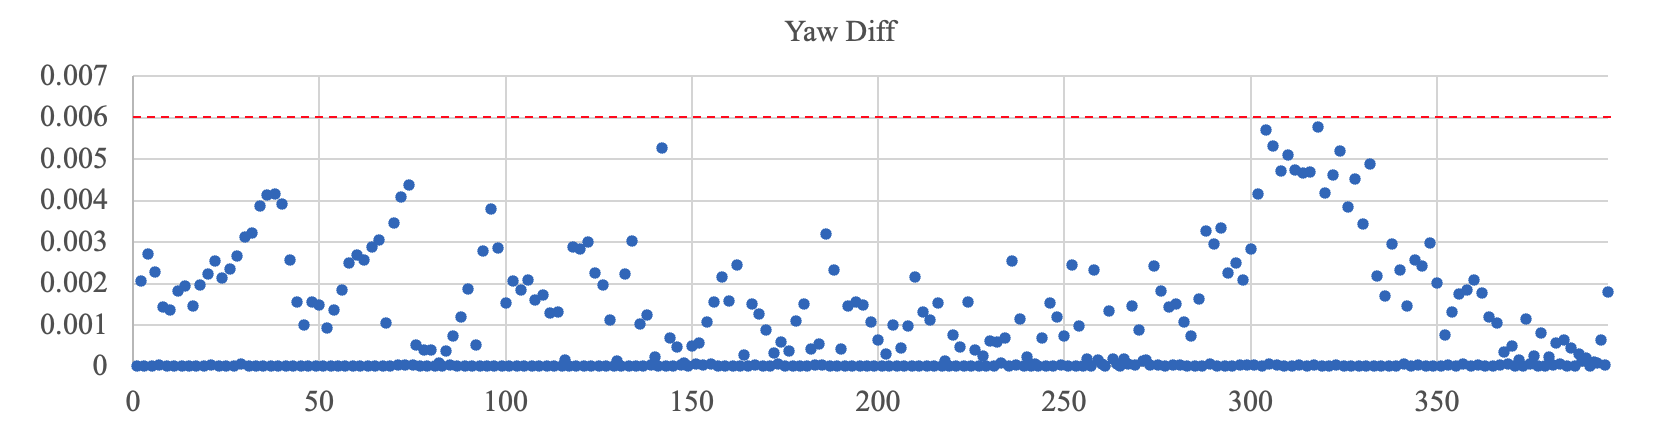
\includegraphics[width=0.8\textwidth]{./res2_icpndtyaw.png}
	\caption{Bag2 NDT減去NDT及ICP切換方法 各別yaw軸數據分析結果(無明顯降低趨勢)}
\end{figure}

\subsection{nuScenes3 result}
由於切換演算法模式精準度還是略差於全NDT方法,在本次並不追求效能上的優化差異最終還是使用NDT方法作為主要演算法,而在第一步可使用NDT作為第一次猜測較佳,綜合上述方法整理以下演算法比較:
\begin{itemize}
	\item Init guess 重要性: ICP >> NDT 
	\item Robust : NDT >> ICP
	\item 精準度: NDT > ICP (Init guess is not good)
	\item 效能:ICP >> NDT
\end{itemize}
由於上述方法對於IMU所提供的數據為原始數據,未經過磁力偏移校正等問題,在此參數轉彎處上對於tracking的Init guess不佳,因此在此bag使用EKF方法進行定位,共進行兩次濾波第一次濾波由IMU及wheel odom做感測融合後,在將經由Lidar的姿態轉換至車輛上與odom filter進行融合,將融合結果為下一次Init guess,在此能有效改善轉彎處誤差,但IMU orientation無covariance濾波結果應該不是最佳結果圖,若要在提升精準度應該需要加入covariance,EKF pipeline 如圖下所示,

\begin{figure}[H]
\centering
	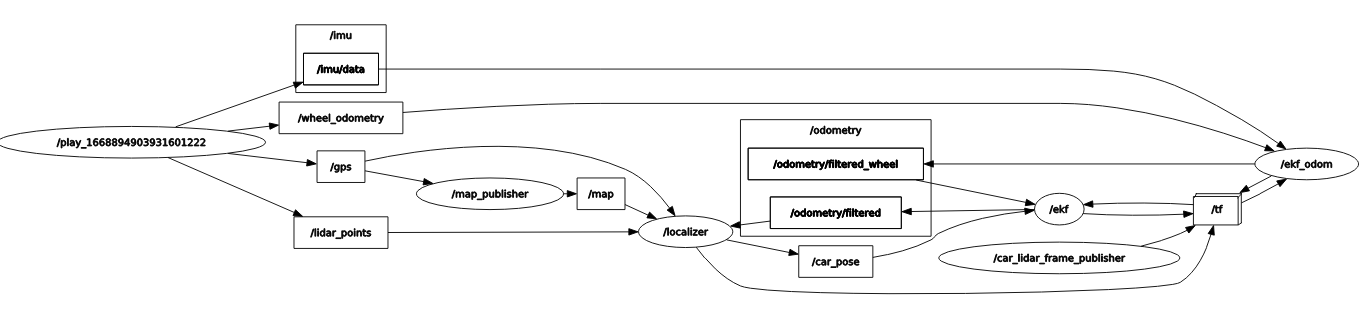
\includegraphics[width=1.0\textwidth]{./ekf_data.png}
	\caption{EKF pipeline}
\end{figure}

\begin{figure}[H]
\centering
	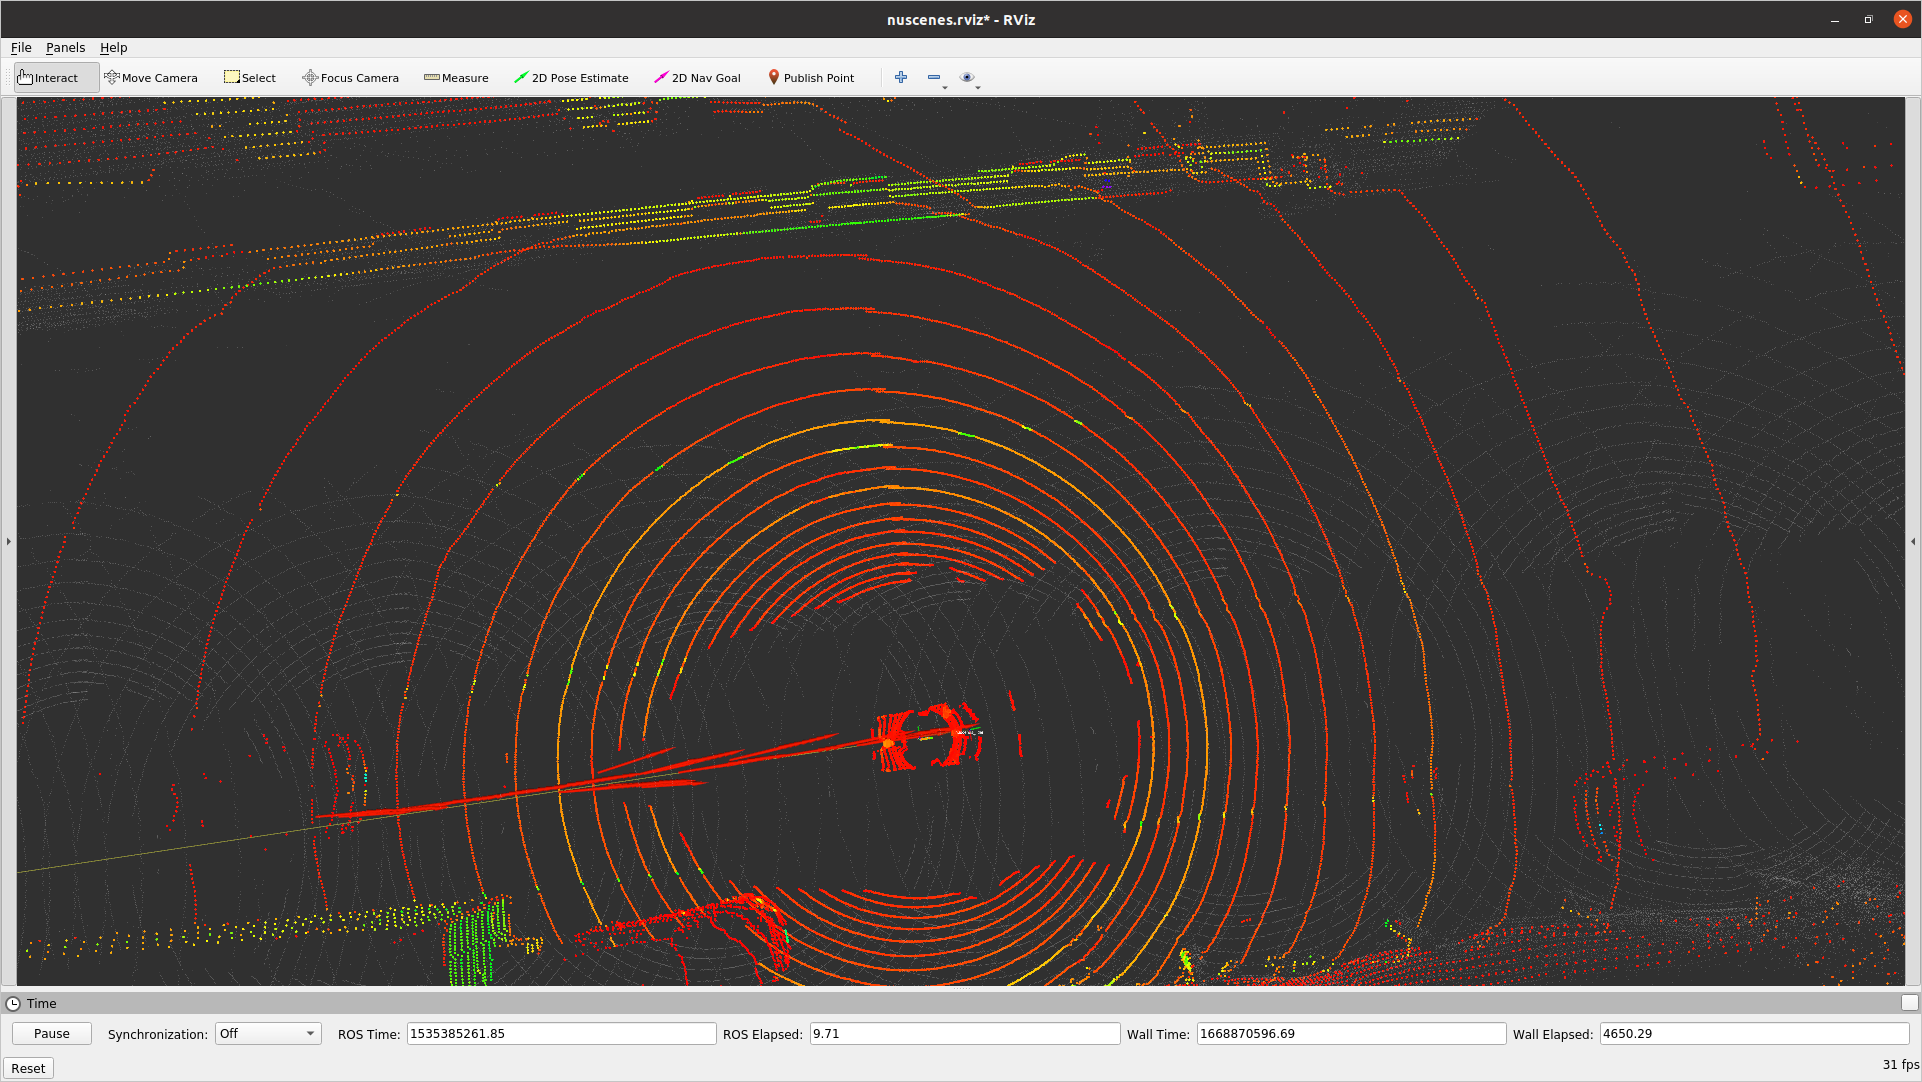
\includegraphics[width=0.8\textwidth]{./ekf_orientation.png}
	\caption{Orientation 濾波不佳問題}
\end{figure}
\section{Problem and Solution}
1.由於採用使用NDT方法需要計算相當久的時間,因此在Bag播放時間過快會導致timestamp無法同步,在雲點圖計算出現跳幀現象導致數據需要重跑,因此使用NDT時採用播放0.5s讓其計算完成才依序播放0.5s,因此耗時大概一個工作天左右,雖然NDT理論上需要較長計算時間,但計算時間超乎想像的久亦有可能是參數設定過於緊導致問題。\\
2.在前幾步誤差較大原因為使用ICP方法需要較好的Init guess 但剛起步是猜測的uncertainty較大因此在前五步可使用NDT作為前幾幀方法,後續經由EKF濾波後可使用ICP方法提高運行速度。
\begin{thebibliography}{1}
 
\bibitem{1}
    Labbe, R. (2014). Kalman and bayesian filters in python. Chap, 7(246), 4.
\end{thebibliography}


\end{document}
